% \documentclass[a4paper, technote, compsoc]{IEEEtran}
\documentclass[../../thesis.tex]{subfiles}

\newcommand{\inner}[2]{\left<#1, #2\right>}
\newcommand{\alemap}{\ensuremath{\mathcal{A}}}
\newcommand{\dt}{\ensuremath{\Delta t}}
\newcommand{\pexp}{\ensuremath{\frac{2\gamma}{\left(\gamma-1\right)}}}
\newcommand{\aleX}{\ensuremath{\mathcal{X}}}
\newcommand{\Ah}[1]{\ensuremath{\vb{#1}^{n+1}_h}}
\newcommand{\Ahn}[1]{\ensuremath{\vb{#1}^{n}_h}}

\newcommand{\rbV}{\ensuremath{\mathbb{V}}}
\newcommand{\rbVT}{\ensuremath{\rbV^T}}
\newcommand{\epspod}{\ensuremath{\varepsilon_\text{POD}}}

\begin{document}

\section{Results and Certification}
\label{sec:results_and_certification}
We are now going to see the Hyperreduced Order Model in action.
The error decay for the solution and the nonlinear operator 
are presented and commented in Section~\ref{sec:hrom_results_reduced_basis}.
% we will study the interaction between the approximation errors
% from the RB and the nonlinear operator bases.

Finally, in Section~\ref{sec:hrom_results_posteriori_error_estimation} we show 
how to certify the HROM solution with a model truncation technique.  

\subsection{Approximation Error}
\label{sec:hrom_results_reduced_basis}
We explore how the number of modes influences the approximation error of the FOM solution.

We have trained our model with 10 samples such that
\begin{align*}
    u_p \sim \frac{\delta \omega L_0}{a_0},
    \nonumber
    \\
    0.15 \leq u_p \leq 0.4,
\end{align*}
to make sure no wiggles appeared and 
that the complete range of system responses were included.

This lead to the following number of basis for each operator,
% Please add the following required packages to your document preamble:
% \usepackage{booktabs}
\begin{table}[!h]
    \caption{For each operator,
    basis size after the tree walk and final size after tree walk compression.
    The nonlinear term and the RB space have the same size, 
    since the RB elements were used to evaluated the nonlinear term.}
    \centering
    \begin{tabular}{@{}rcc@{}}
    \toprule
                      & After Treewalk & Final \\ \midrule
    RB                & 295            & 69                \\
    RHS               & 20             & 2                 \\
    Mass              & 10             & 1                 \\
    Stiffness         & 10             & 1                 \\
    Nonlinear         & 690            & 69                \\
    Convection        & 20             & 2                 \\
    Nonlinear-Lifting & 10             & 1                 \\ \bottomrule
    \end{tabular}
\end{table}

Since we are using a POD to build our reduced basis, 
we attempt to relate the POD a posteriori error estimations with 
the actual error between ROM and FOM.

\subsubsection{POD: A Posteriori Errors}
The POD returns a collection of vectors and sigular values, 
$(\psi_i(x), \sigma_i)$,
each related to the other.
The magnitude of each singular value $\sigma_i$ somehow encodes 
how much information is carried by its associated vector about the original span.
% Departing from the idea that we need at least \textit{one} basis element to solve our problem,
% and that we have a finite amount of 

We define the energy of the basis that contains up to the $i$-th element as
\begin{equation}
    \mathcal{E}_i = \frac{\sum_{j=0}^{i}\sigma_j^2}{\sum \sigma_k^2}.
\end{equation}
This magnitude is derived from the \textit{a posteriori} error bounds 
for a POD reconstruction, where the following inequality holds,
\begin{equation}
    \norm{y(x) - \sum_{j=0}^{n} w_j \psi_j(x)}_{2}^{2} \leq \sum_{i = n+1}^{N} \sigma_i^2,
\end{equation}
with $y(x)$ belonging to the snapshots matrix used to build the POD basis.
This inequality is telling us that if up to~$n$ basis vectors are used
to reconstruct a vector belonging to the original span,
the average error in the $L_2$ sense will be smaller or equal
to the sum of the remaining squared singular values.

We shall see if this variable has any predictive power on the ROM error.

\subsubsection{Error Decay}
We want to find the smallest size $N^{*}$ for which the FOM is correctly reproduced.
Naturally, the exact value of this variable is problem-dependent, 
but the way in which we approach its search would suit any RB problem.

We have done this online simulation for one sample, 
for a location in the parameter space where the system response is the most nonlinear.
\begin{table}[h]
    \centering
    \caption{Online sampling parameters, 
    sorted in ascending order by piston mach~$u_p$ values.}
    \begin{tabular}{cccc}
    \toprule
        $a_0$ & $\omega$ & $\delta$ & $u_p$
        \\ \midrule
        22.96 &   29.55 & 0.15 &           0.20 \\
        19.28 &   22.87 & 0.20 &           0.23 \\
        18.24 &   18.88 & 0.29 &           0.30 \\
        24.64 &   27.13 & 0.29 &           0.32 \\
        20.62 &   25.98 & 0.29 &           0.37
        \\ \bottomrule
    \end{tabular}
\end{table}

In Figure~\ref{fig:error_decay} we present the ROM error with respect to 
the number of basis elements and the energy of the truncated basis.
\begin{figure}[h]
    \centering
    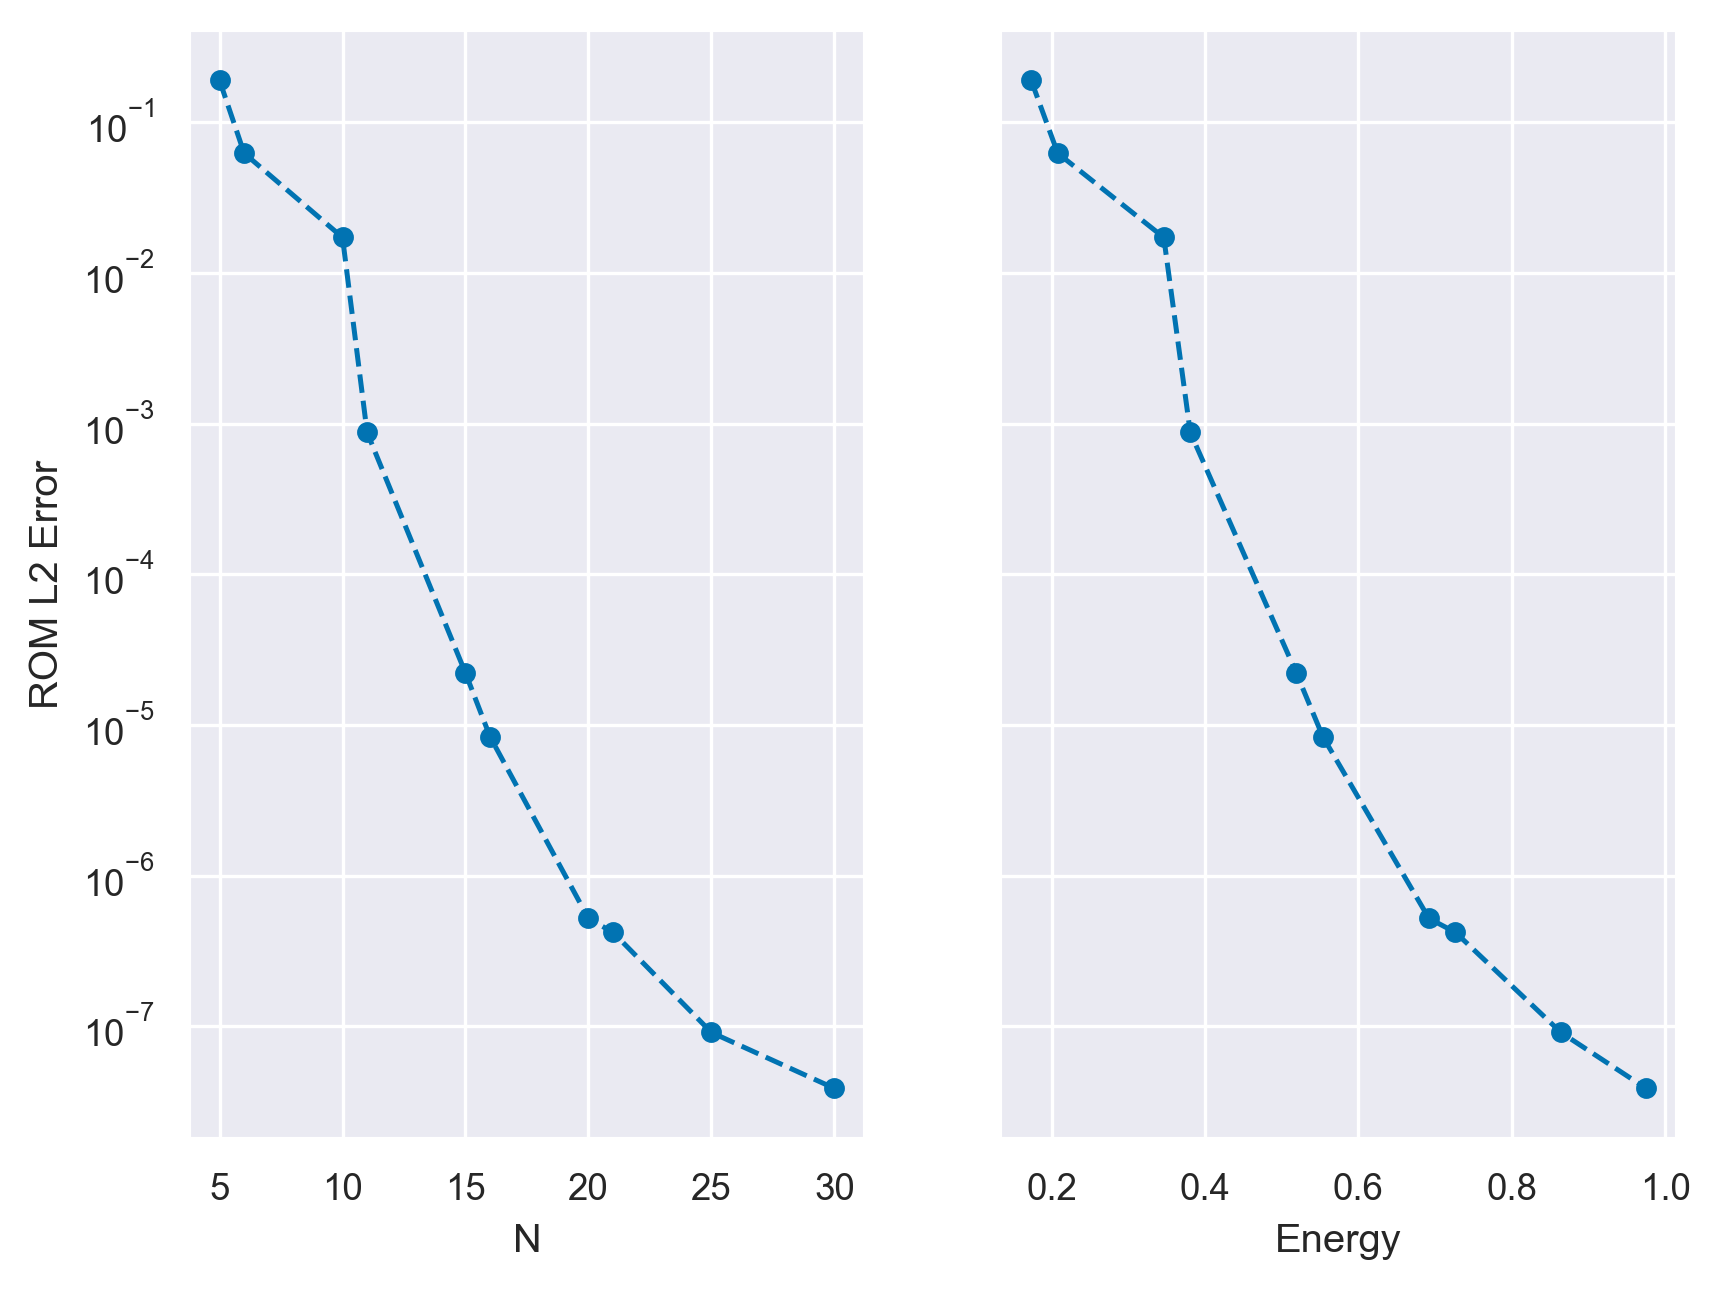
\includegraphics[width=\columnwidth]{research_project/piston/figures/rb_certification/error_decay.png}
    \caption{Error decay for number of basis elements and basis energy level.
    Expectedly, the more basis elements we have, the lower the error.}
    \label{fig:error_decay}
\end{figure}
The more elements in the basis, the smaller the error.
The more energy the basis contains, the better the approximation.

We present in Figures~\ref{fig:outflow_model_comparison_N_5} 
and \ref{fig:outflow_model_comparison_N_10} 
the actual solution at the outflow for each model (FOM and ROM).
We can see how the ROM model is poorly resolved for $N=5$, as reflected by the error,
but how it drastically improves for $N=10$, except for the initial instants of movement.
\begin{figure}[h]
    \centering
    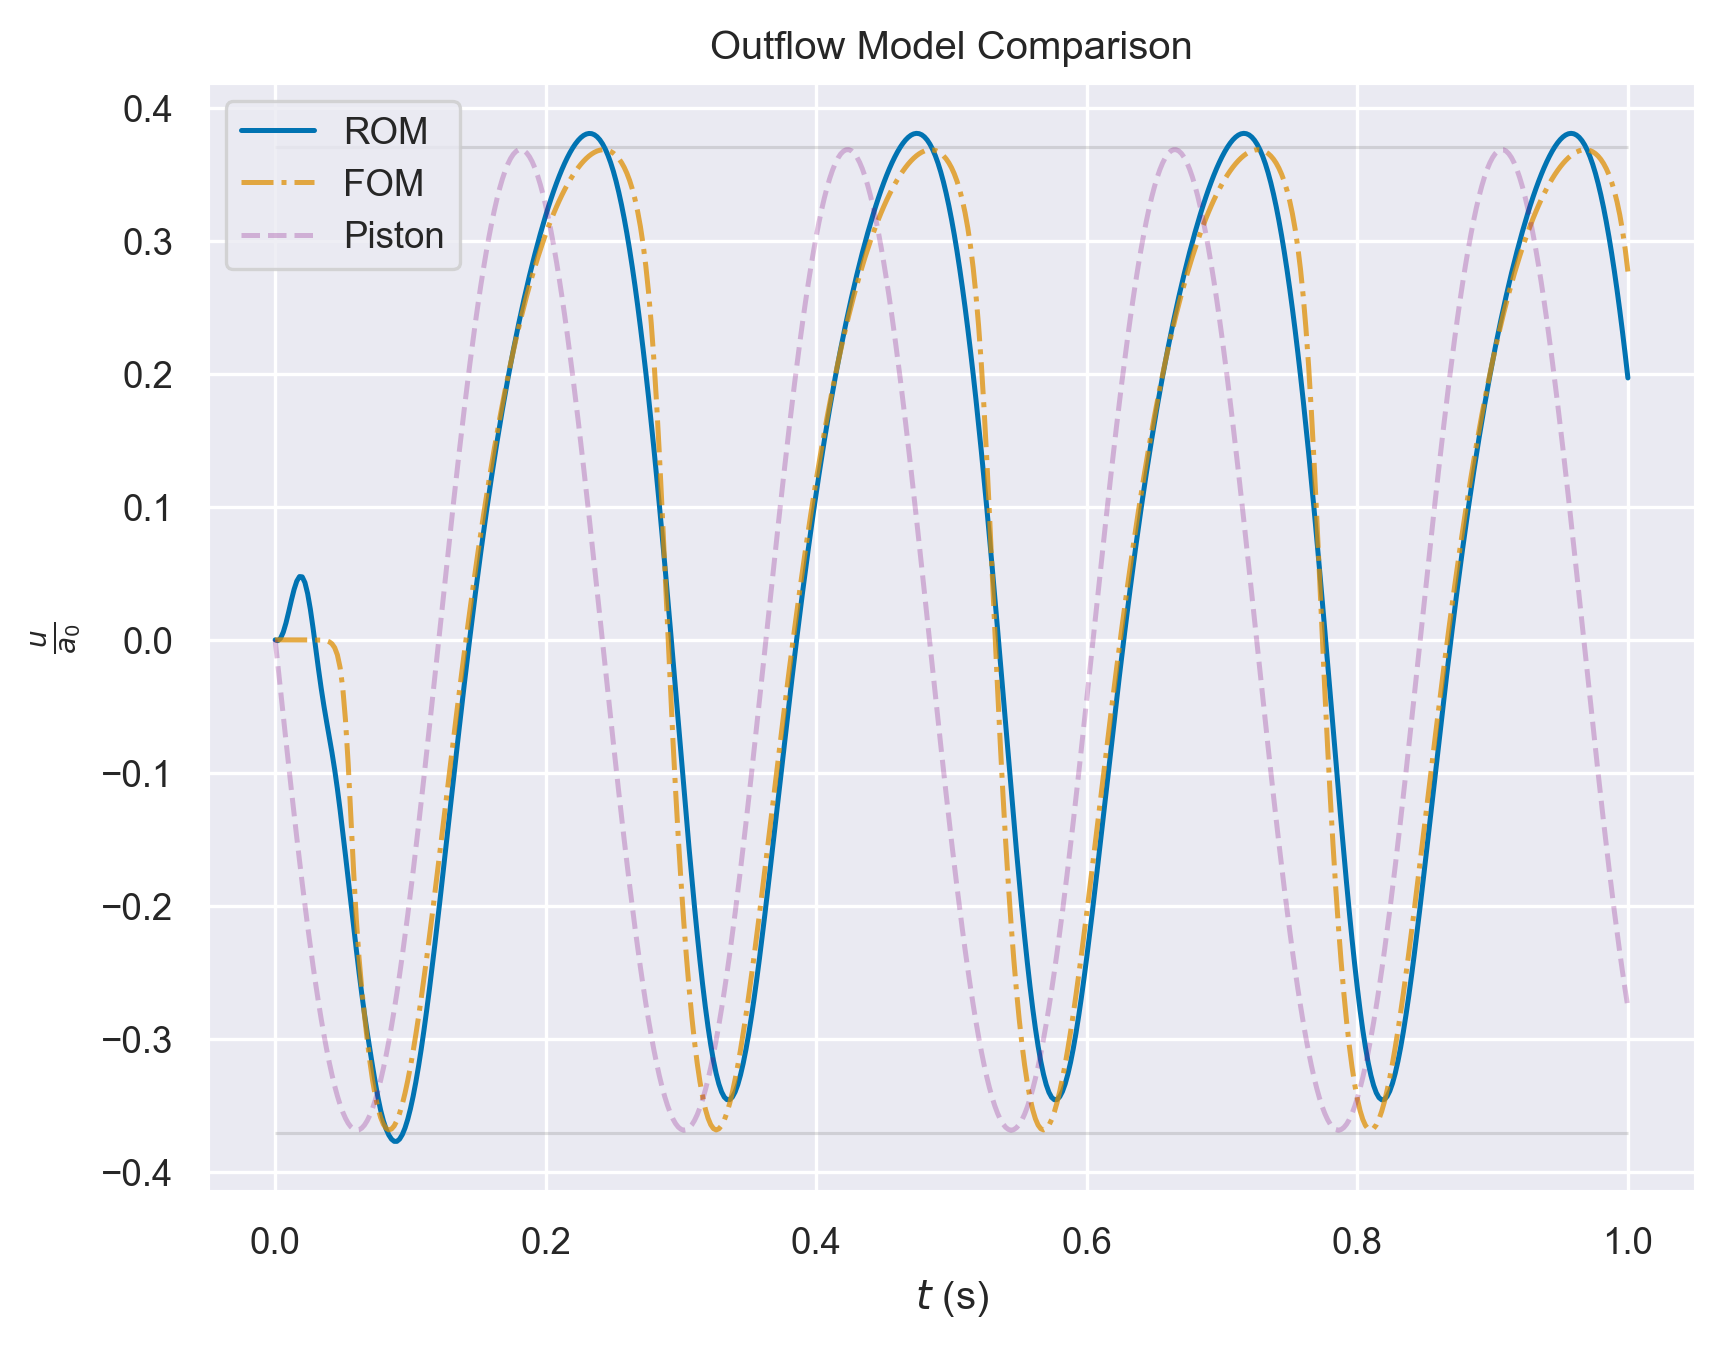
\includegraphics[width=\columnwidth]{research_project/piston/figures/rb_certification/outflow_probes_comparison_rom_5_srom_15_online_4.png}
    \caption{Outflow velocities for different models. The ROM model is poorly resolved for $N=5$.}
    \label{fig:outflow_model_comparison_N_5}
\end{figure}
\begin{figure}[h]
    \centering
    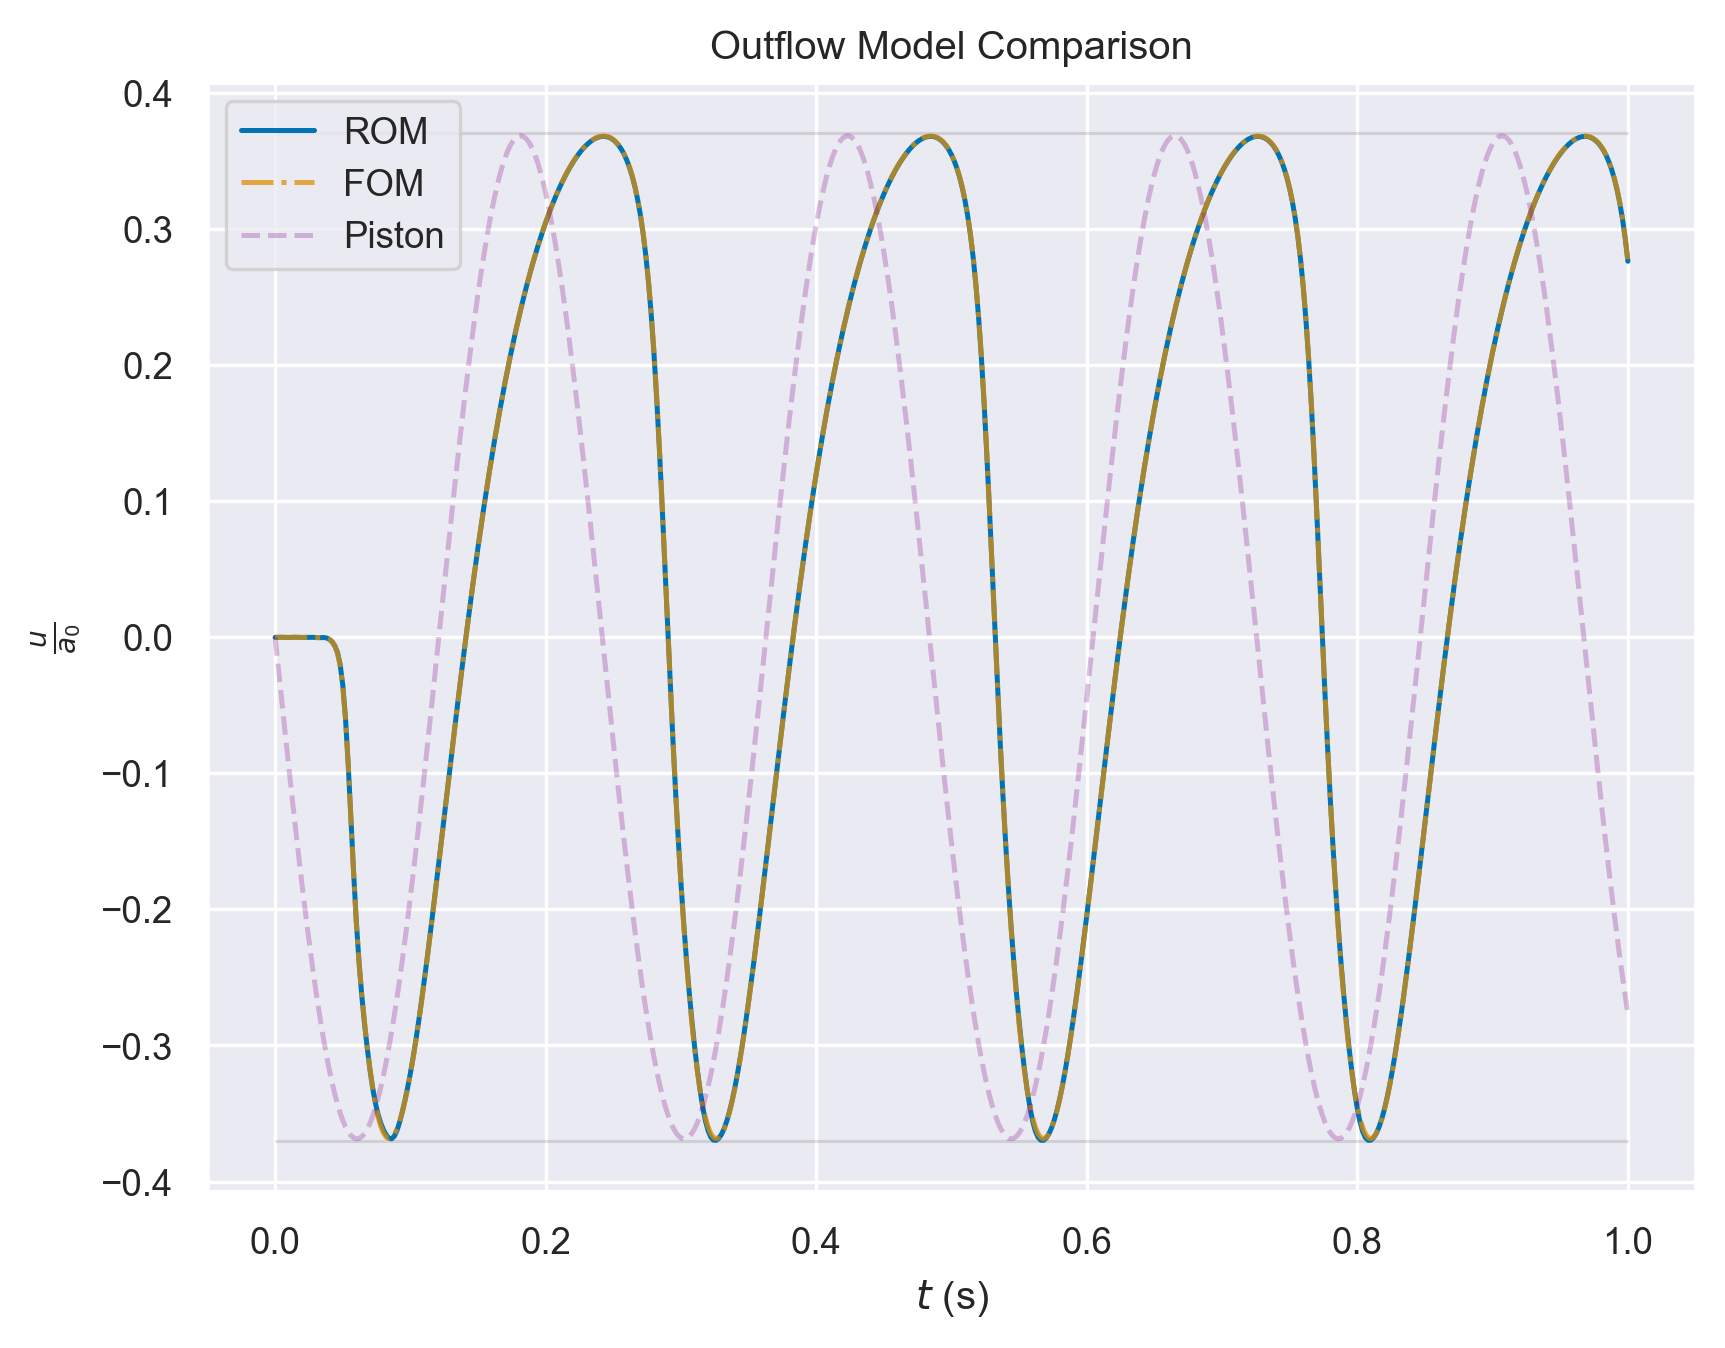
\includegraphics[width=\columnwidth]{research_project/piston/figures/rb_certification/outflow_probes_comparison_rom_10_srom_20_online_4.png}
    \caption{Outflow velocities for different models. 
    The ROM model is better resolved for $N=10$, except at the beginning of the simulation.}
    \label{fig:outflow_model_comparison_N_10}
\end{figure}
The flow departs from rest as the piston starts to move.
Therefore, the first snapshots contain a nonlinearity in the sense that the flow starts to move on one side, 
but remains still along the rest of the tube.

However, for most of the time interval, this kind of nonlinearity will not be present again,
since the flow will be in constant motion, flowing in and out of the system.
Hence, it is an expected behaviour that this is the interval where the ROM will fail the most,
unless we include a sufficient number of basis elements.
To fix this problem, certain techniques exist which enhance the POD basis 
without adding excessive complexity \cite{weightedPOD}.

\subsection{(M)DEIM Error Estimation}
\mytodo{HROM Results: Show how to reduce $\min / \max$ weak forms.
This will be a proxy to show that other stabilization schemes suit this technique.}
In this section we are going to explore the reduction of the nonlinear operator.

In Figure~\ref{fig:mdeim_error_approximation} we show the mean approximation error
in time for the nonlinear operator. 
The first ten elements of the reduced basis were used to assemble the operators.
We see that unless the complete basis is used ($N=69$),
the approximation error is quite poor.
\begin{figure}[h]
    \centering
    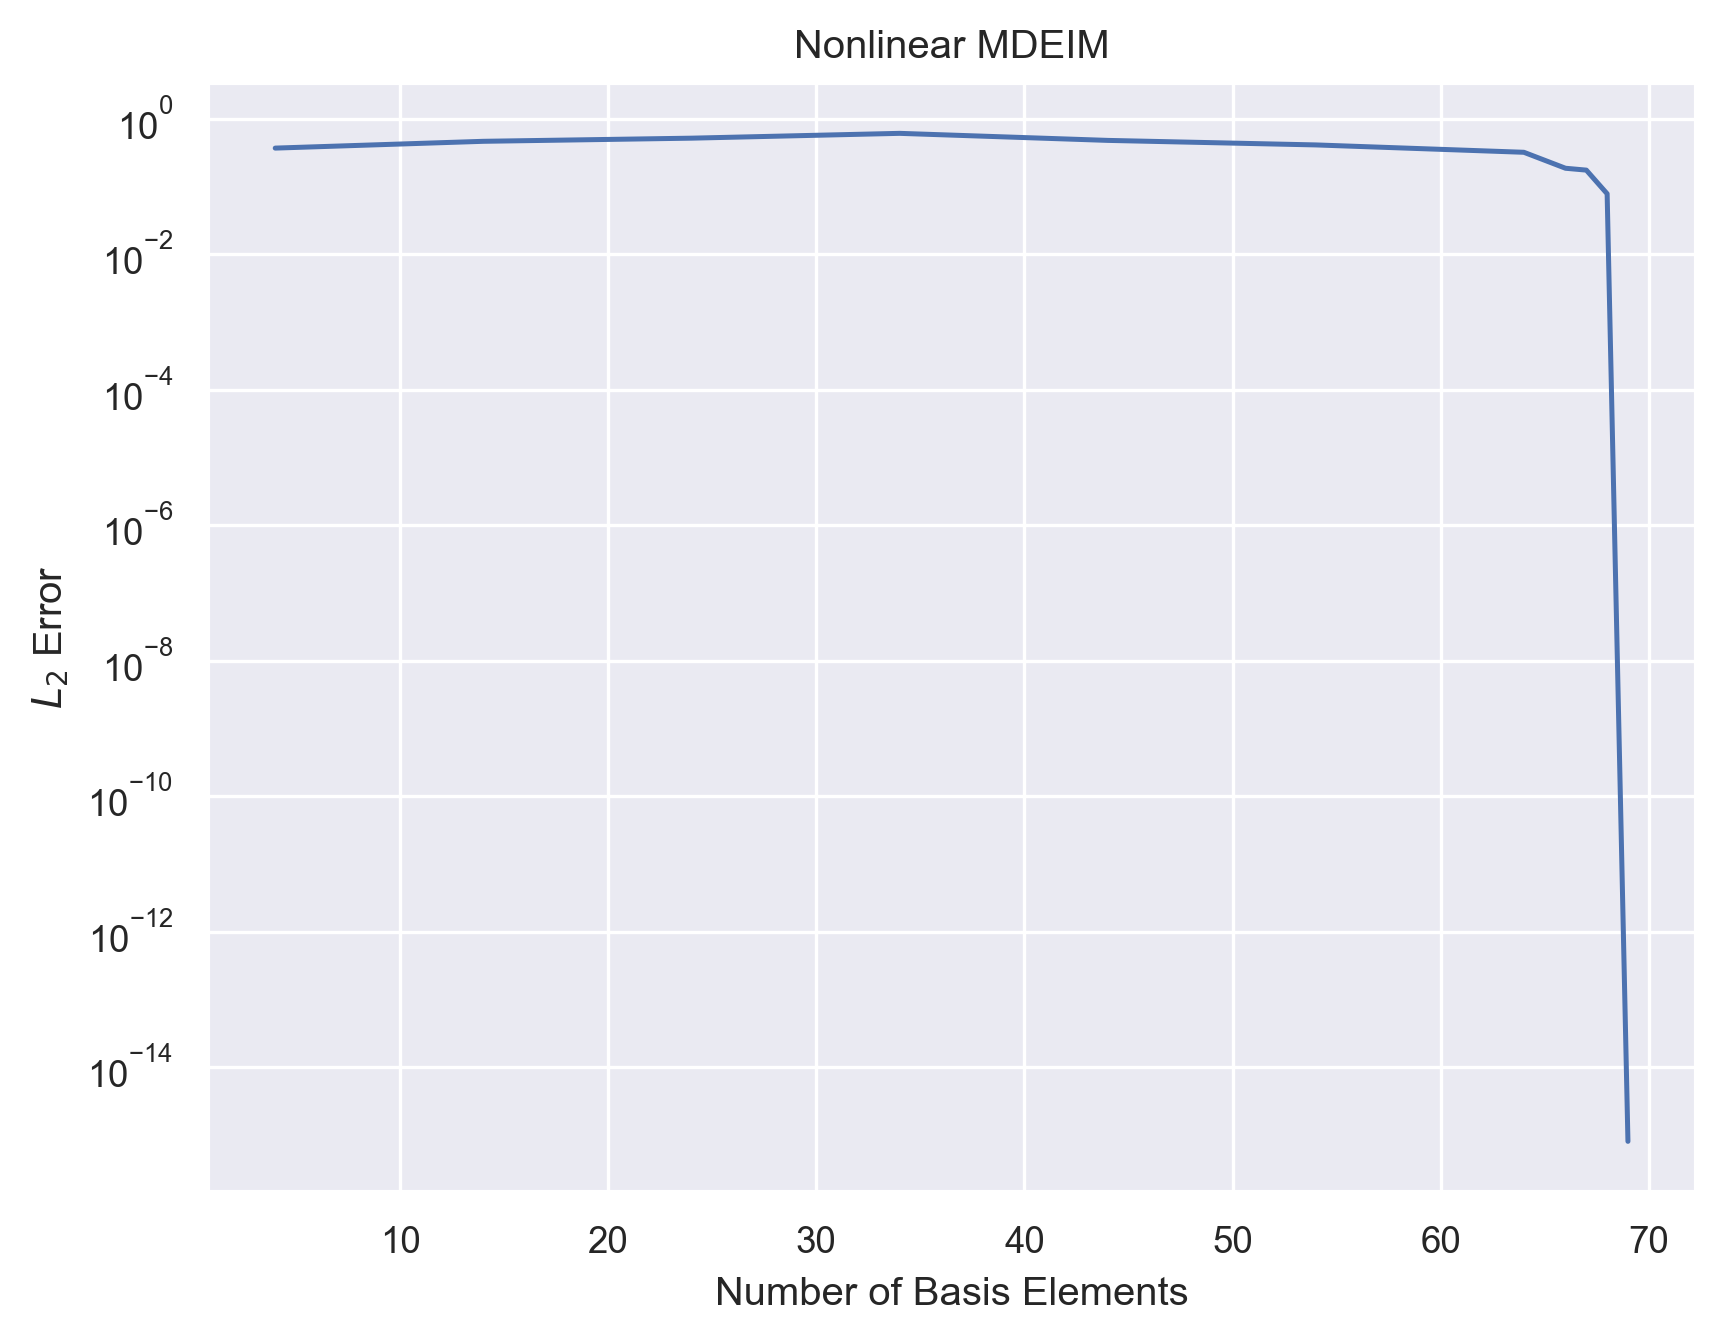
\includegraphics[width=1\columnwidth]{research_project/piston/figures/mdeim_certification/nonlinear_error_decay.png}
    \caption{Nonlinear MDEIM error approximation for incremental number of elements in the basis.
    The first ten elements of the reduced basis were used to assemble the operator.
    The approximation is quite poor, unless the complete basis is used 
    ($N=69$).}
    \label{fig:mdeim_error_approximation}
\end{figure}

We believe this has to do with the fact that the reduced basis elements,
which form an orthogonal basis, were used to assemble the nonlinear operator snapshots.
Hence, all the POD basis elements contain fundamental information,
as hinted by the abrupt drop in the singular value, see Figure~\ref{fig:sigmas_decay}. 
\begin{figure}[h]
    \centering
    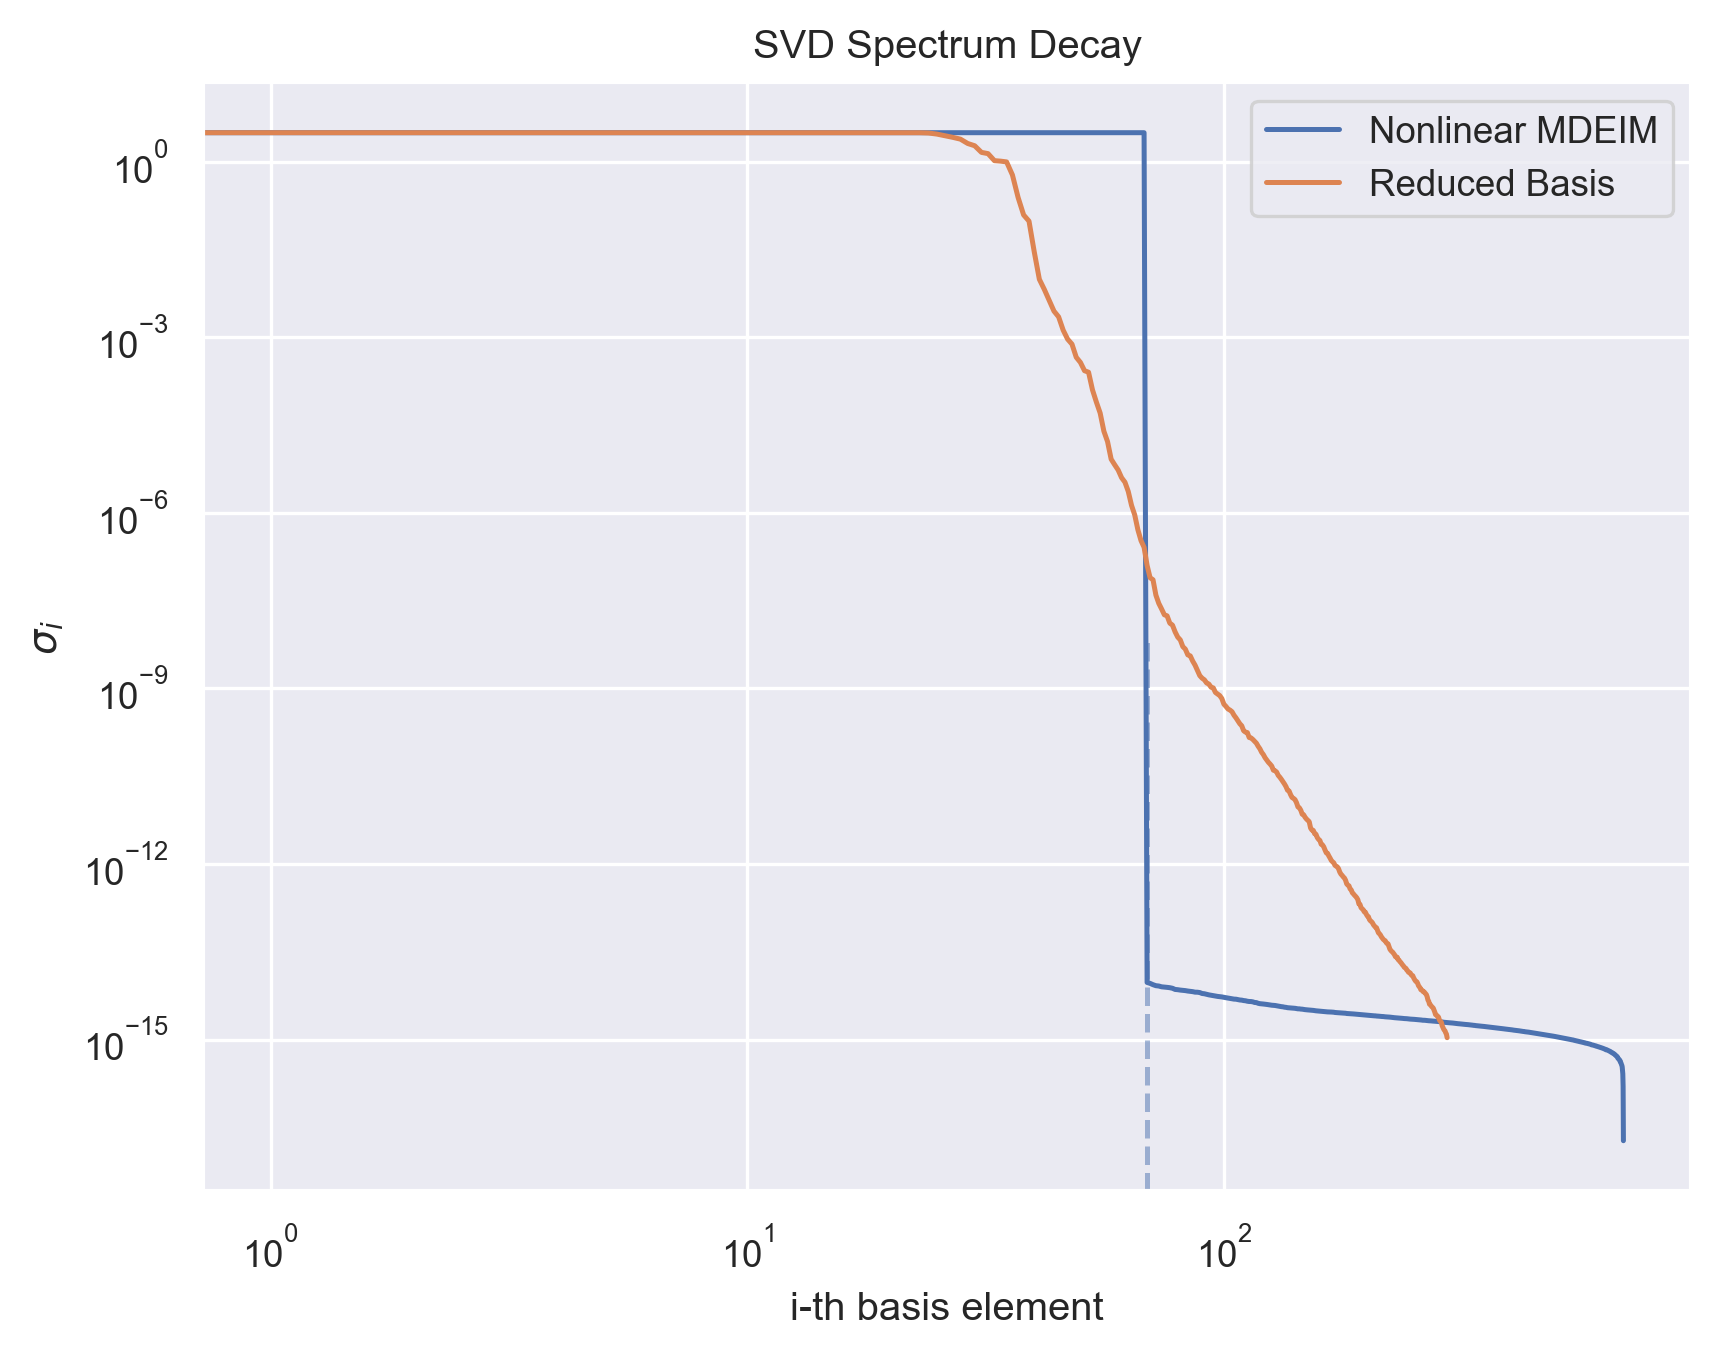
\includegraphics[width=1\columnwidth]{research_project/piston/figures/mdeim_certification/sigmas_problem.png}
    \caption{Singular values decay for the reduced basis and the nonlinear operator.
    The dashed vertical line corresponds to the number of reduced basis elements, $N=69$.
    The basis for the nonlinear operator does not present the same pattern as the 
    one for the reduced basis.
    All of the elements of the nonlinear operator basis 
    seem to contain the same amount of information from the span.
    We believe this has to do with the fact that the reduced basis elements,
    which form an orthogonal basis, were used to assemble the nonlinear operator snapshots.}
    \label{fig:sigmas_decay}
\end{figure}

In the light of these results, 
we necessarily need to use the whole MDEIM basis for our simulations.

\subsubsection{Hierarchical Basis}
The previous results show that the basis obtained using
snapshots built with the RB basis elements is not hierarchical.
This is an unconvenient result.

Although the assembly of the nonlinear operator has been simplified
in terms of computational costs,
there are no degrees of freedom to adjust the reconstruction error,
which is a common operation in the field of Reduced Models.

Hence, we explore an alternative approach, collecting nonlinear term snapshots 
during the simulation of the FOM, and compressing them with the same 
nested strategy as we did for the reduced basis.

By doing so, we do recover a hierarchical basis, which allows us to tune the error,
as proved by the singular value decay (Figure~\ref{fig:sigmas_decay_from_fom}).
The basis for the nonlinear operator presents the same pattern 
as the solution reduced basis.
We believe this has to do with the fact that the linearized nonlinear operator is a trilinear form.
Hence, due to the simplicity of the Jacobian, the reduction difficulty is similar to the one
required for the reduced basis.
\begin{figure}[h]
    \centering
    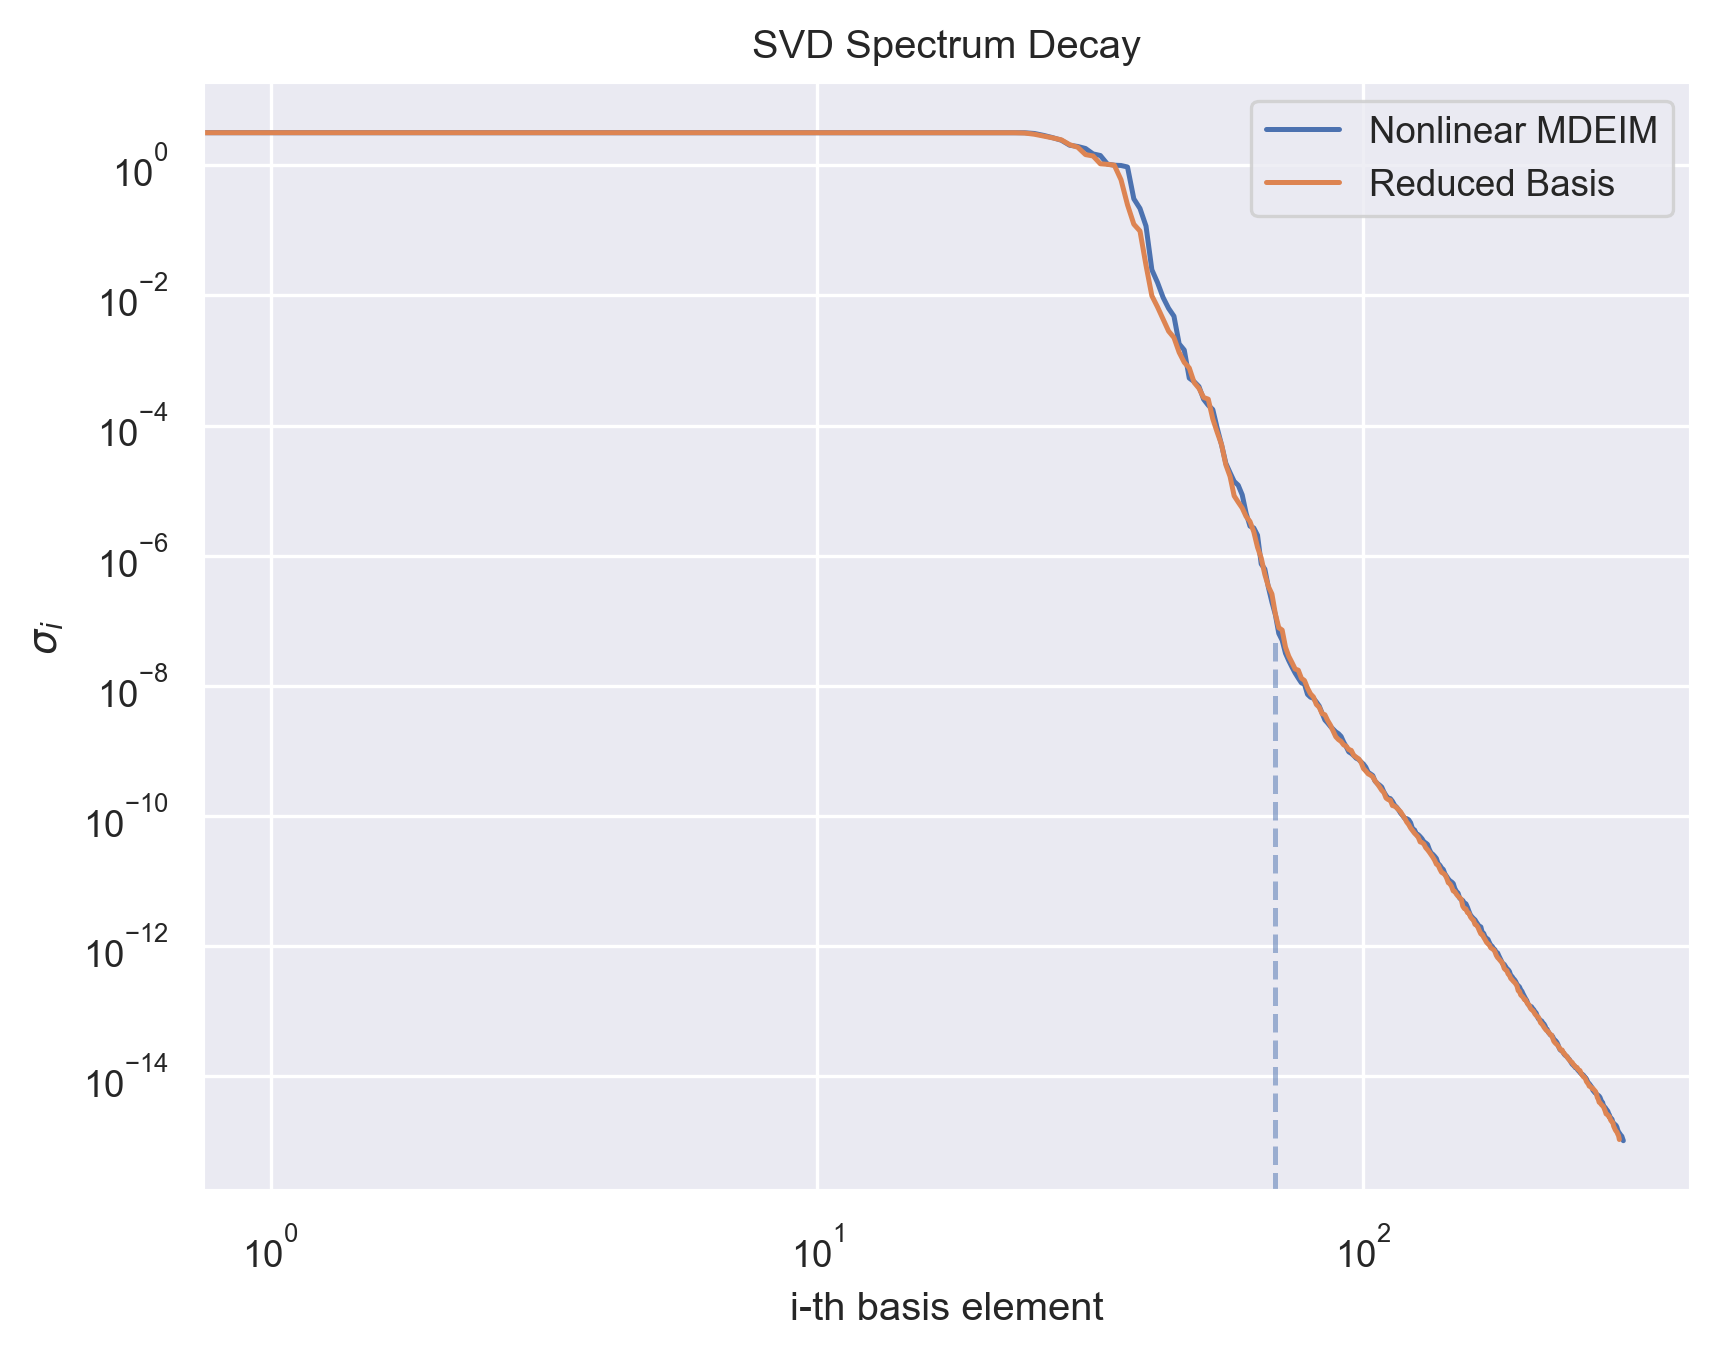
\includegraphics[width=1\columnwidth]{research_project/piston/figures/mdeim_certification/sigmas_problem_from_fom.png}
    \caption{Singular values decay for the reduced basis and the nonlinear operator.
    The dashed vertical line corresponds to the number of basis elements, $N=70$.
    The basis for the nonlinear operator presents the same pattern 
    (and hence the same size)
    as the solution reduced basis.
    We believe this has to do with the fact that the linearized nonlinear operator is a trilinear form.
    Hence, due to the simplicity of the Jacobian, the reduction difficulty is similar to the one
    required for the reduced basis.}
    \label{fig:sigmas_decay_from_fom}
\end{figure}

In Table~\ref{tab:mdeim_certification} we show the parameter range for which
we tested this alternative basis against the first ten reduced basis elements
(for which we averaged the error).
\begin{table}[h]
    \centering
    \caption{Parameter space for nonlinear term reconstruction.}
    \label{tab:mdeim_certification}
    \begin{tabular}{cccc}
        \toprule
        $a_0$  & $\omega$ & $\delta$ & $u_p$ \\
        \midrule
        24.275 &  18.549  & 0.203 &  0.155 \\
        21.055 &  15.969  & 0.236 &  0.179 \\
        23.627 &  24.427  & 0.211 &  0.218 \\
        21.533 &  24.376  & 0.200 &  0.226 \\
        20.440 &  18.913  & 0.289 &  0.267 \\
        23.849 &  27.396  & 0.261 &  0.300 \\
        19.976 &  23.190  & 0.259 &  0.301 \\
        20.633 &  24.184  & 0.280 &  0.329 \\
        18.803 &  29.705  & 0.226 &  0.357 \\
        19.890 &  27.986  & 0.278 &  0.391 \\
        \bottomrule
\end{tabular}
\end{table}

In Figures~\ref{fig:nonlinear_error_decay_from_fom_by_parameter} and~\ref{fig:nonlinear_error_decay_from_fom}
we present the reconstruction error decay, as the N-MDEIM basis is truncated.
This time, the basis does show the expected error decay as modes are removed,
hence allowing to speed up even further computations if some compromise is made in the error.

\begin{figure}[h]
    \centering
    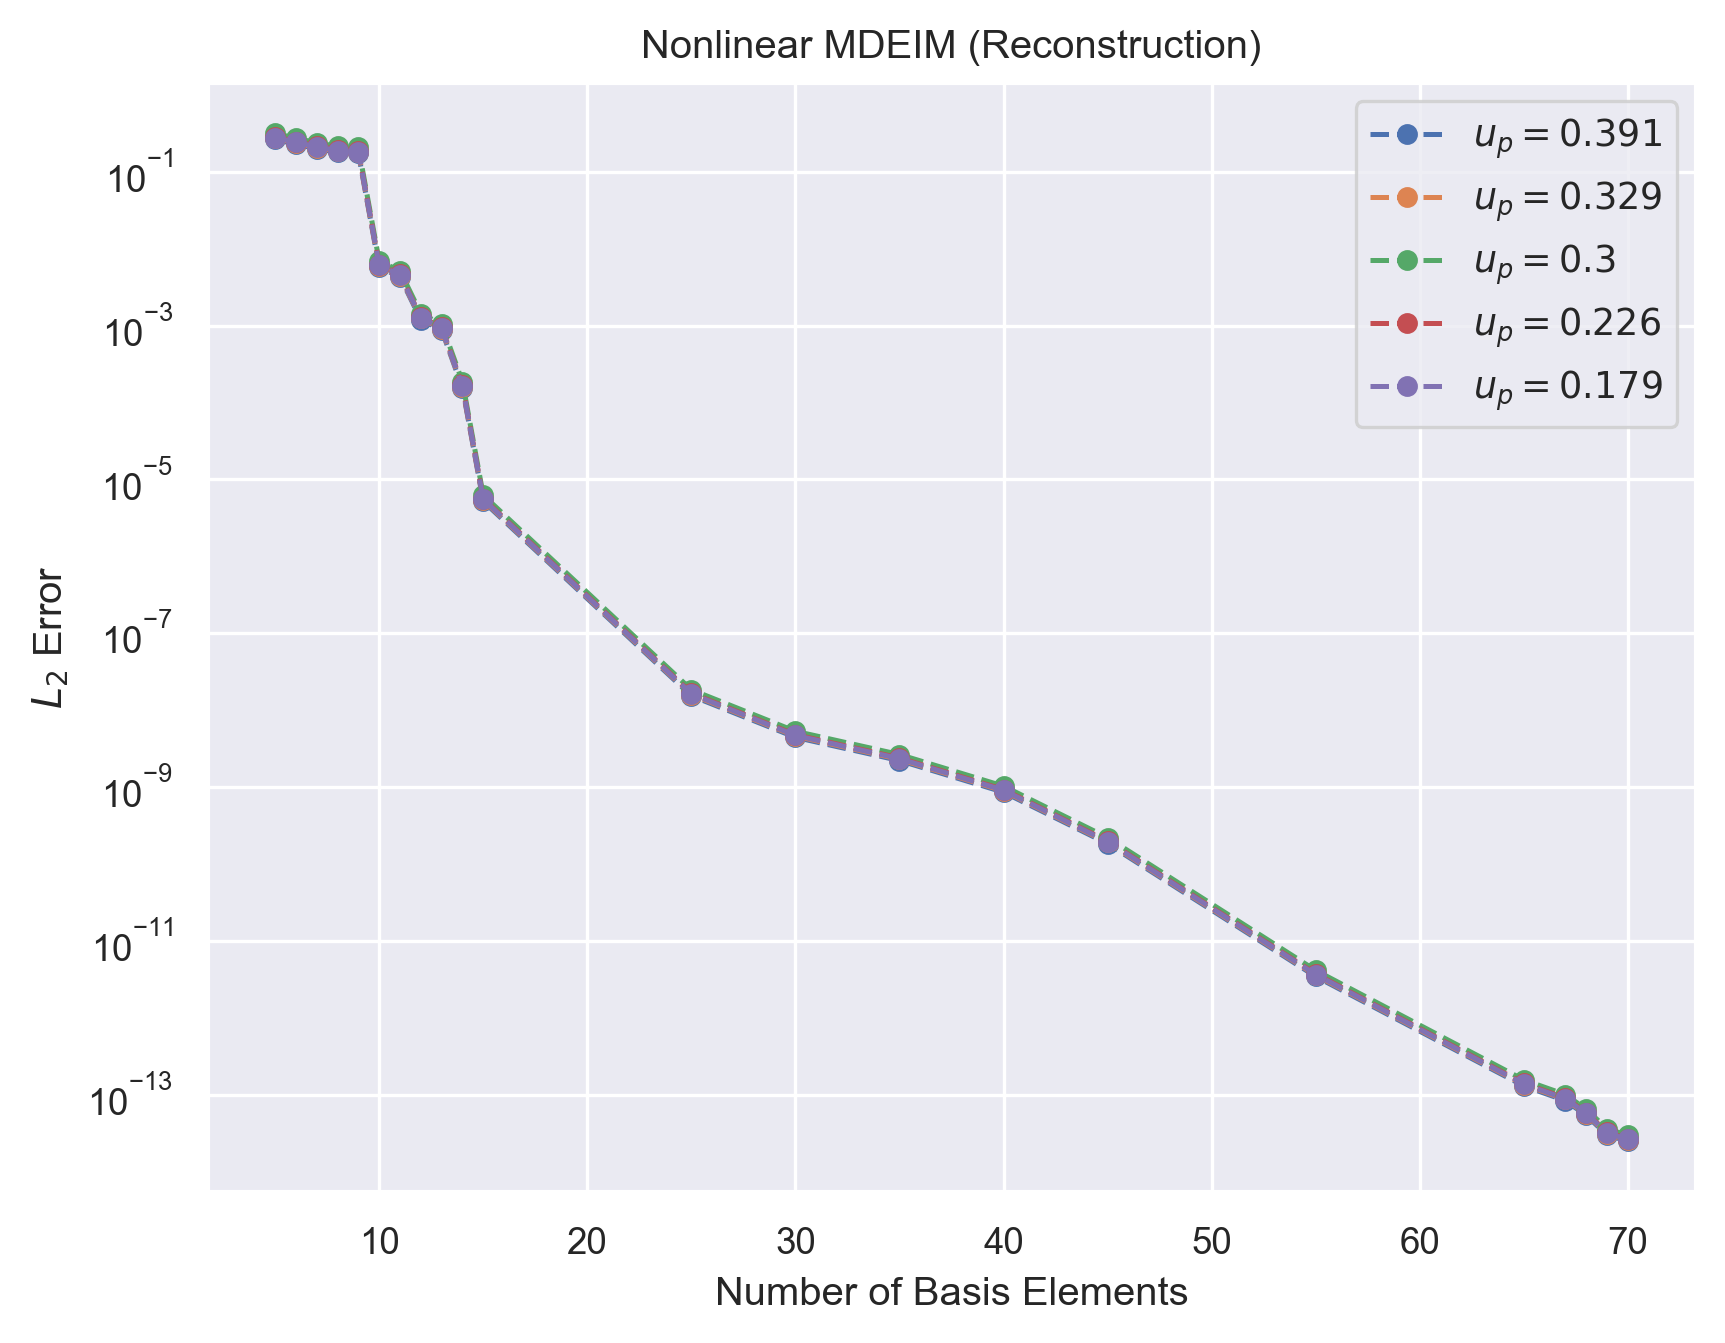
\includegraphics[width=1\columnwidth]{research_project/piston/figures/mdeim_certification/nonlinear_error_decay_by_parameter.png}
    \caption{N-MDEIM reconstruction error decay, as we truncate the modes from the MDEIM basism
    for some individual parametrizations.
    Probably due to the simplicity of the problem, Jacobian and the fact that the linearized term is trilinear in
    all of its arguments, there is no noticeable difference for different parametrizations.}
    \label{fig:nonlinear_error_decay_from_fom_by_parameter}
\end{figure}

\begin{figure}[h]
    \centering
    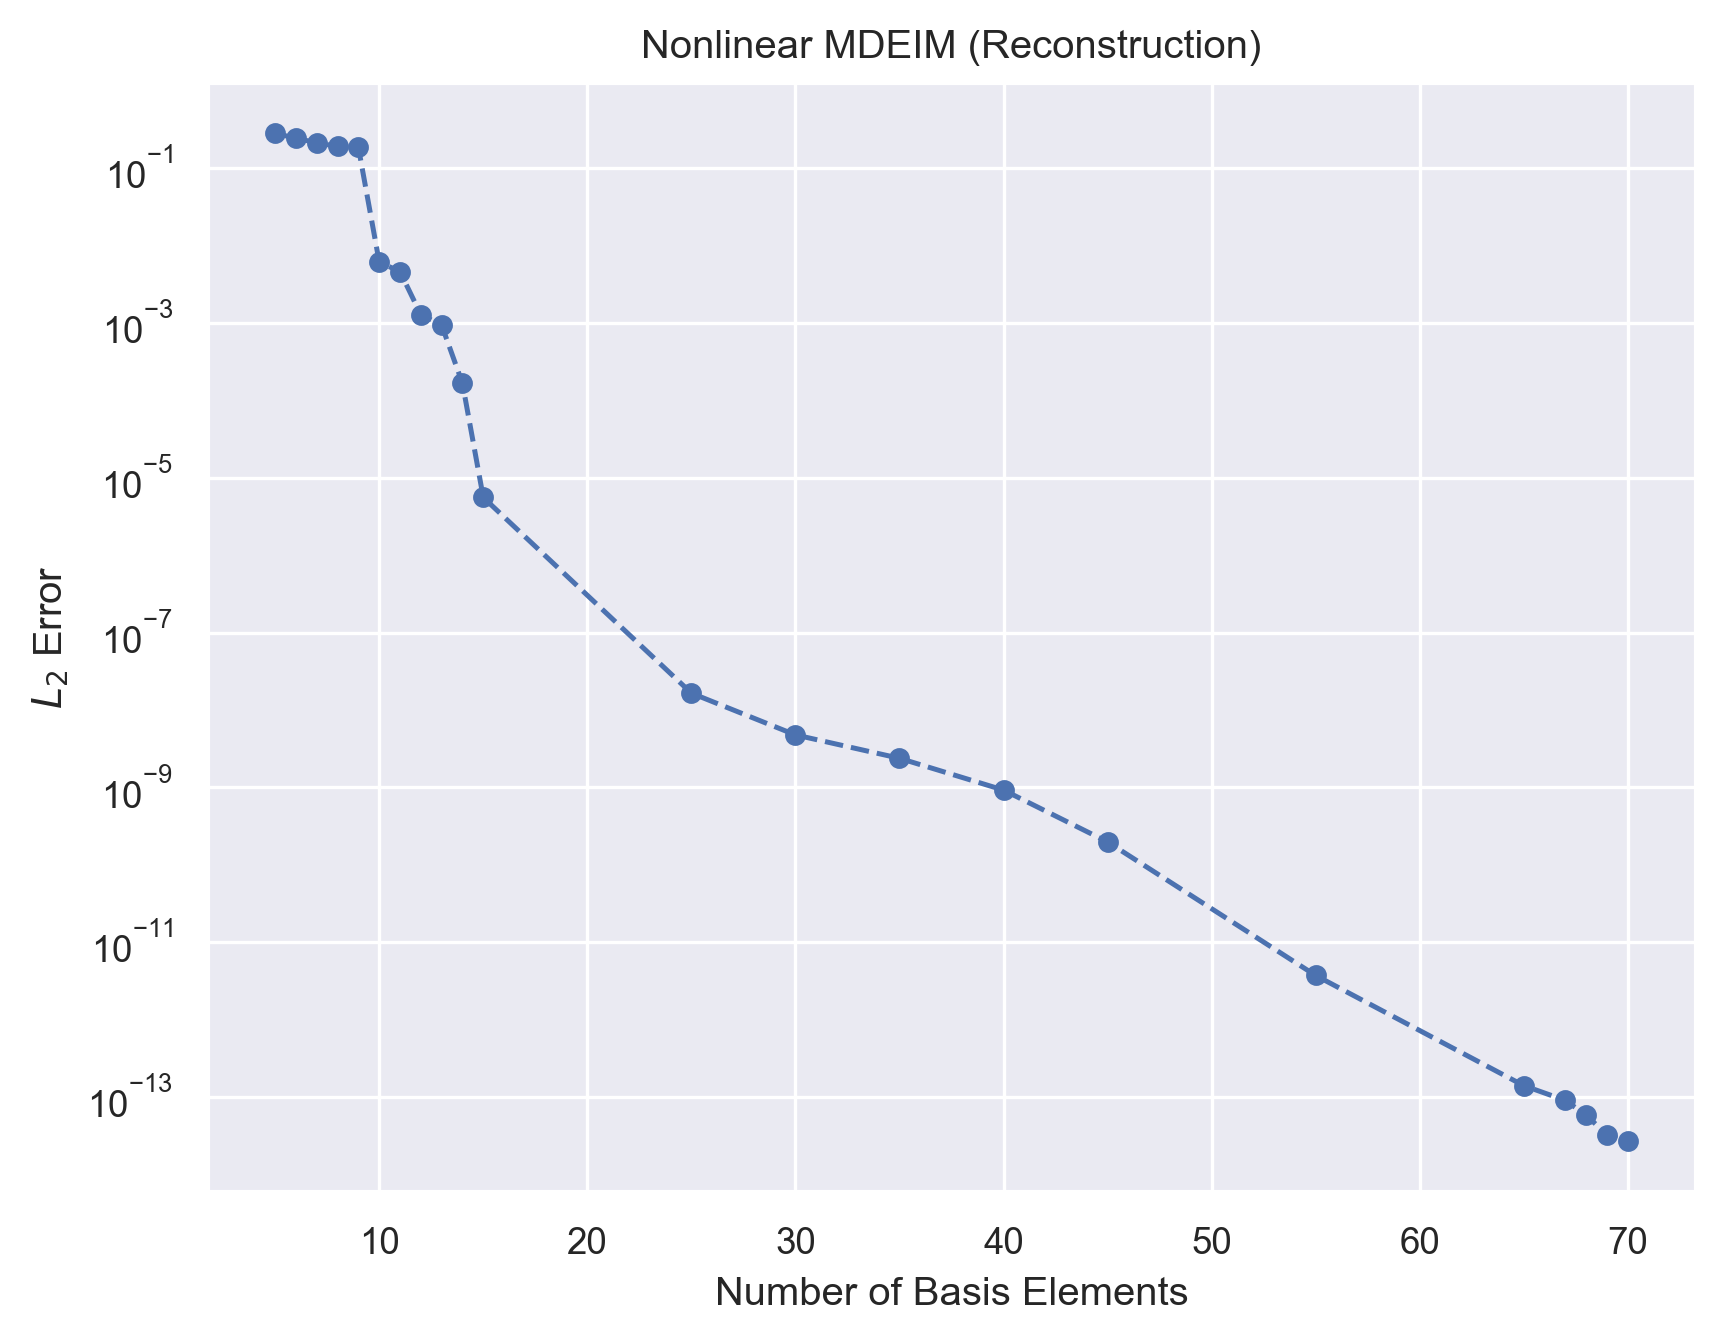
\includegraphics[width=1\columnwidth]{research_project/piston/figures/mdeim_certification/nonlinear_error_decay_from_fom.png}
    \caption{N-MDEIM reconstruction error decay, as we truncate the modes from the MDEIM basis, averaged across parametrizations.}
    \label{fig:nonlinear_error_decay_from_fom}
\end{figure}

\subsubsection{Reduced Basis and MDEIM Error Interaction}
Finally, we truncate both bases (solution and nonlinear operator spaces)
simultaneously, to determine the interaction between both of them.
In Table~\ref{tab:nonlinear_error_decay_heatmap} we present 
the timewise $L_2$ error for different numbers of reduced basis 
and nonlinear operator basis elements.
In Figure~\ref{fig:nonlinear_error_decay_heatmap} we present the same table,
albeit in a heatmap plot. 

Expectedly, we reach a situation where one error dominates the other one,
that is, increasing the number of elements for one basis will not improve the
results unless the other one is enlarged too.
If we wanted to achieve a determined error threshold,
we would have to analyze and take into account all the operator errors simultaneously.
\begin{table}[h]
    \centering
    \caption{Timewise $L_2$ error decay for different truncation levels 
    of the reduced basis space (N) 
    and the nonlinear operator basis (N-MDEIM).}
    \begin{tabular}{ccccccc}
        \toprule
        N-MDEIM &      5  &      10 &      15 &      30 &      40 &      50 \\
        N  &         &         &         &         &         &         \\
        \midrule
        5  & 3.4e-2 & 3.4e-2 & 3.4e-2 & 3.4e-2 & 3.4e-2 & 3.4e-2 \\
        10 & 3.4e-3 & 7.8e-4 & 7.8e-4 & 7.8e-4 & 7.8e-4 & 7.8e-4 \\
        15 & 3.3e-3 & 2.1e-5 & 1.4e-5 & 1.4e-5 & 1.4e-5 & 1.4e-5 \\
        20 & 3.3e-3 & 1.7e-5 & 8.0e-7 & 7.8e-7 & 7.8e-7 & 7.8e-7 \\
        25 & 3.3e-3 & 1.7e-5 & 2.8e-7 & 1.5e-7 & 1.5e-7 & 1.5e-7 \\
        30 & 3.3e-3 & 1.7e-5 & 2.5e-7 & 5.1e-8 & 5.3e-8 & 5.3e-8 \\
        35 & 3.3e-3 & 1.7e-5 & 2.5e-7 & 4.5e-8 & 4.6e-8 & 4.6e-8 \\
        \bottomrule
    \end{tabular}
    \label{tab:nonlinear_error_decay_heatmap}
\end{table}

\begin{figure}[h]
    \centering
    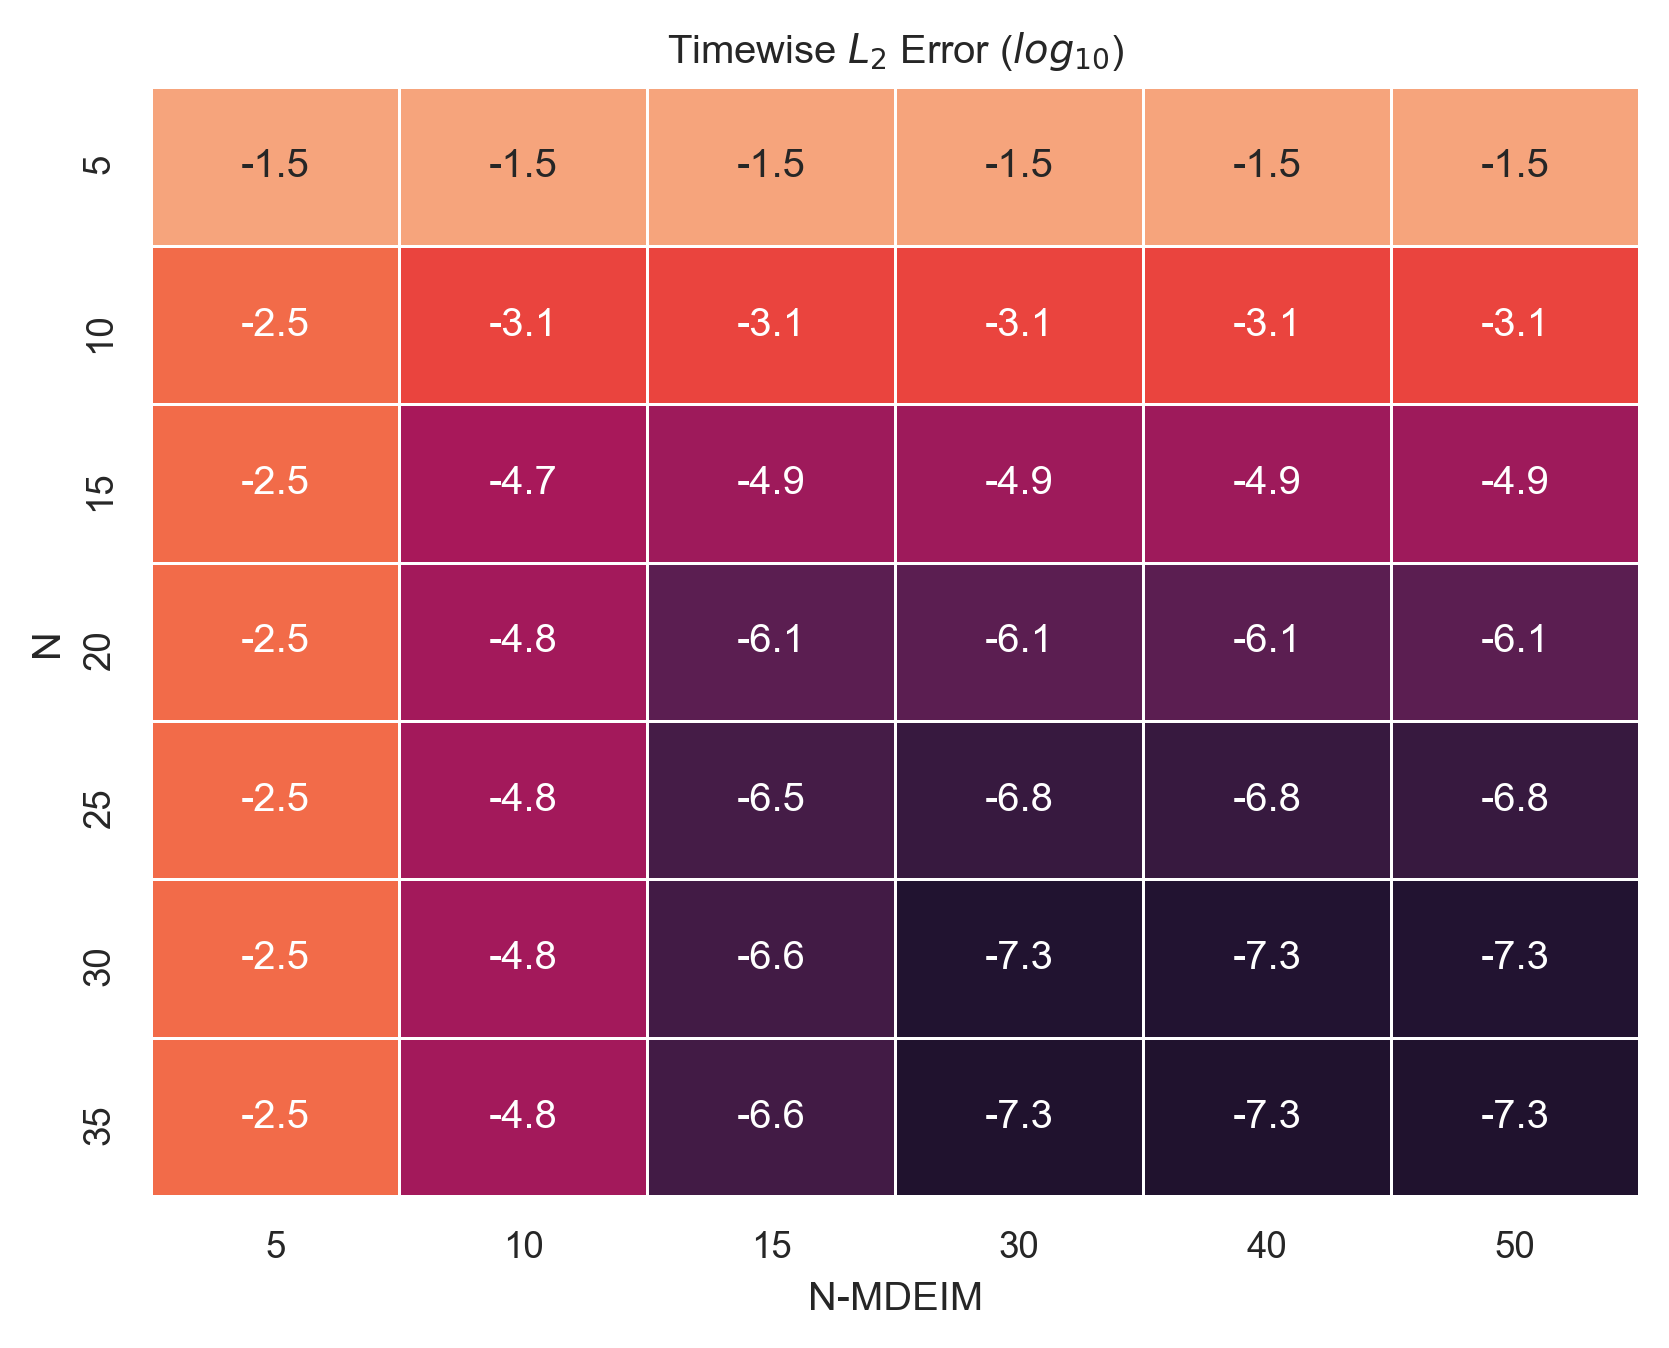
\includegraphics[width=1\columnwidth]{research_project/piston/figures/mdeim_certification/error_decay_heatmap.png}
    \caption{Timewise $L_2$ error decay for different truncation levels 
    of the reduced basis space (N) 
    and the nonlinear operator basis (N-MDEIM).
    The $log_{10}$ transformation was applied, so that the heatmap color gradient is smooth.}
    \label{fig:nonlinear_error_decay_heatmap}
\end{figure}

\subsection{HROM Error Estimation}
\label{sec:hrom_results_posteriori_error_estimation}
To compute the HROM error in the preceding sections
we required the assembly and solution of the FOM model.
This is an undesirable fact, since if to validate our ROM solution
we need to compute its FOM counterpart, 
we are better off computing straightaway the FOM model 
(which will be absolutely accurate).

Hence, we need an efficient a posteriori error estimator.

\subsubsection{Sacrificial ROM}
We use the \textit{model truncation} technique.
That is, we are going to carry with us \textit{two} ROMs,
with different basis elements.

The second one, called \textit{sacrificial} ROM (SROM),
will be used to compute the actual error for the base ROM,
without requiring the calculation of the FOM.
\mytodo{SROM: Create descriptive flow chart.}
The SROM is baptized with such name because its results cannot be used,
since we have no way to estimate their error.
We assume it is smaller than the one of base ROM, since it has more basis elements,
but we cannot know how much smaller it is.
Hence, it is an additional ROM whose results we use to estimate the error of the former, 
and nothing else.

For this error estimation procedure, the question we seek answering is:
\textit{how many more nodes needs the SROM to carry to certify with accuracy the base ROM?}
Again, the answer to this question is problem-dependent,
but our approach to find it could be used for any other problem.

\subsubsection{Error Estimation}
We depart from the error we seek to bound,
and proceed to add and susbtract the solution from the sacrificial ROM,
\begin{equation}
    \norm{u_h - \rbV_{N} u_N} = \norm{u_h \pm \rbV_{\hat{N}} u_{\hat{N}} - \rbV_{N} u_{N}},
\end{equation}
where $\hat{N} > N$. 
By the triangle inequality, we get
\begin{equation}
    \norm{u_h - \rbV_{N} u_N} \leq \norm{u_h - \rbV_{\hat{N}} u_{\hat{N}}} + \norm{\rbV_{\hat{N}} u_{\hat{N}} - \rbV_{N} u_{N}}.
\end{equation}
If we define the error function $e_N = \norm{u_h - \rbV_{N} u_N}$, 
we get an upper bound of the desired error in terms of the sacrificial ROM error and the error between ROMs,
\begin{equation}
    e_N \leq e_{\hat{N}} + \norm{\rbV_{\hat{N}} u_{\hat{N}} - \rbV_{N} u_{N}}.
\end{equation}
With sufficient RB elements, it should be safe to assert that the error made 
with additional modes should be smaller or equal to the one made without it,
\begin{equation}
    e_{\hat{N}} \leq e_{N}.
\end{equation}
Thus, we get the following error bound,
\begin{equation}
    e_N \leq \norm{\rbV_{\hat{N}} u_{\hat{N}} - \rbV_{N} u_{N}},
\end{equation}
It remains to determine how sharp this error estimate is.

\subsubsection{Error Between Two ROMs}
The error estimator 
\begin{equation}
    \tilde{e}_{N}(\hat{N}) = \norm{\rbV_{\hat{N}} u_{\hat{N}} - \rbV_{N} u_{N}}
\end{equation}
can be expressed as a sum in terms of the RB elements.
Due to the hierarchical character of the RB basis, $\rbV_{\hat{N}}$ contains the same elements 
up to $N$ as $\rbV_{N}$.
Thus, the error between ROMs can be expressed like
\begin{equation}
    \begin{split}
        \norm{\rbV_{\hat{N}} u_{\hat{N}} - \rbV_{N} u_{N}} 
        = \\ 
        \norm{
        \sum_{i=N+1}^{\hat{N}} u^{\hat{N}}_{i} \psi_{i} 
        + 
        \sum_{j}^{N} (u^{\hat{N}}_{j} - u^{N}_{j}) \psi_j
        }.
    \end{split}
\end{equation}
The difference $(u^{\hat{N}}_{j} - u^{N}_{j})$ between ROM coefficients should be relatively small, 
since it represents the difference between the two coefficients associated to the same mode.
If they were notably different, 
it would mean that the dynamics between the original ROM and the sacrificial one are different.
Since the basis is hierarchical, this effect is unlikely to happen: 
adding an additional mode should only refine the solution, 
not change drastically how the previous modes are scaled.
They are not strictly the same because the ROM matrix changes if more modes are added to the basis,
but again, it does so in a way that dynamics should be preserved.
\mytodo{Plot: Common mode amplitudes for ROM and SROM. 
We expect the coefficients to coincide when a sufficient number of basis elements are included.}

In Figure~\ref{fig:estimator_accuracy_timewise} we show in the behaviour of the error estimator 
for each timestep.
\begin{figure}[h]
    \centering
    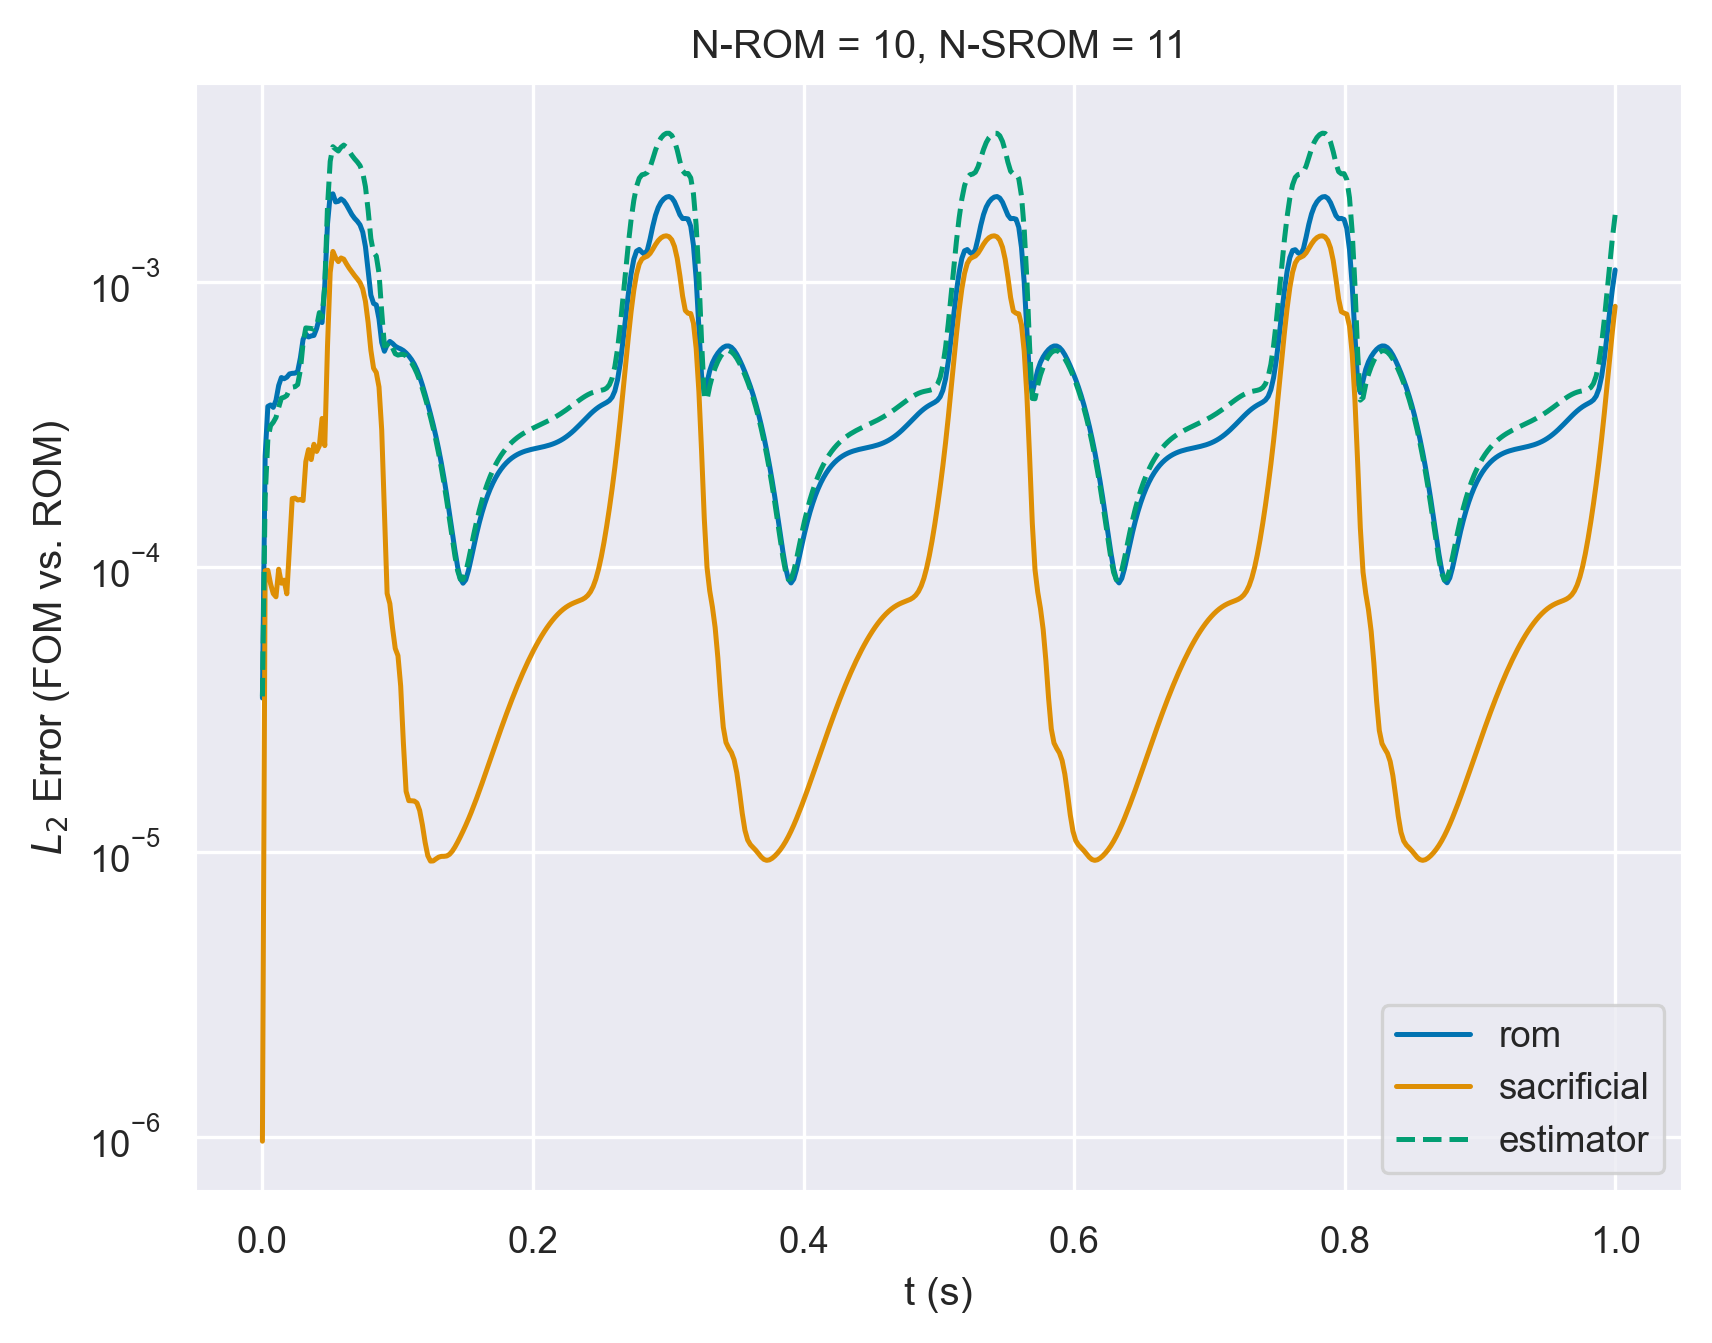
\includegraphics[width=1\columnwidth]{research_project/piston/figures/rb_certification/error_estimation_rom_10_srom_11.png}
    \caption{Time-wise a posteriori error estimator accuracy for $N_{\text{ROM}} = 10$, $N_{\text{SROM}} = 11$.
    We observe how accurate the estimator is carrying only one additional mode.}
    \label{fig:estimator_accuracy_timewise}
\end{figure}
In Figure~\ref{fig:estimator_accuracy} we present how close is the estimator to the actual error,
both aggregated in the time direction.
We have computed the estimator for~\mbox{$\Delta N = 1, 5$} and~$10$ additional modes.
Then, we compute \textit{estimator accuracy}, how far it is from the actual ROM error,
aggregated for all timesteps, 
\mytodo{Esitmator accuracy: make this a relative error.}
\begin{equation}
    \text{Estimator Accuracy} = \norm{e_t - \tilde{e}_t} 
\end{equation}
\begin{figure}[h]
    \centering
    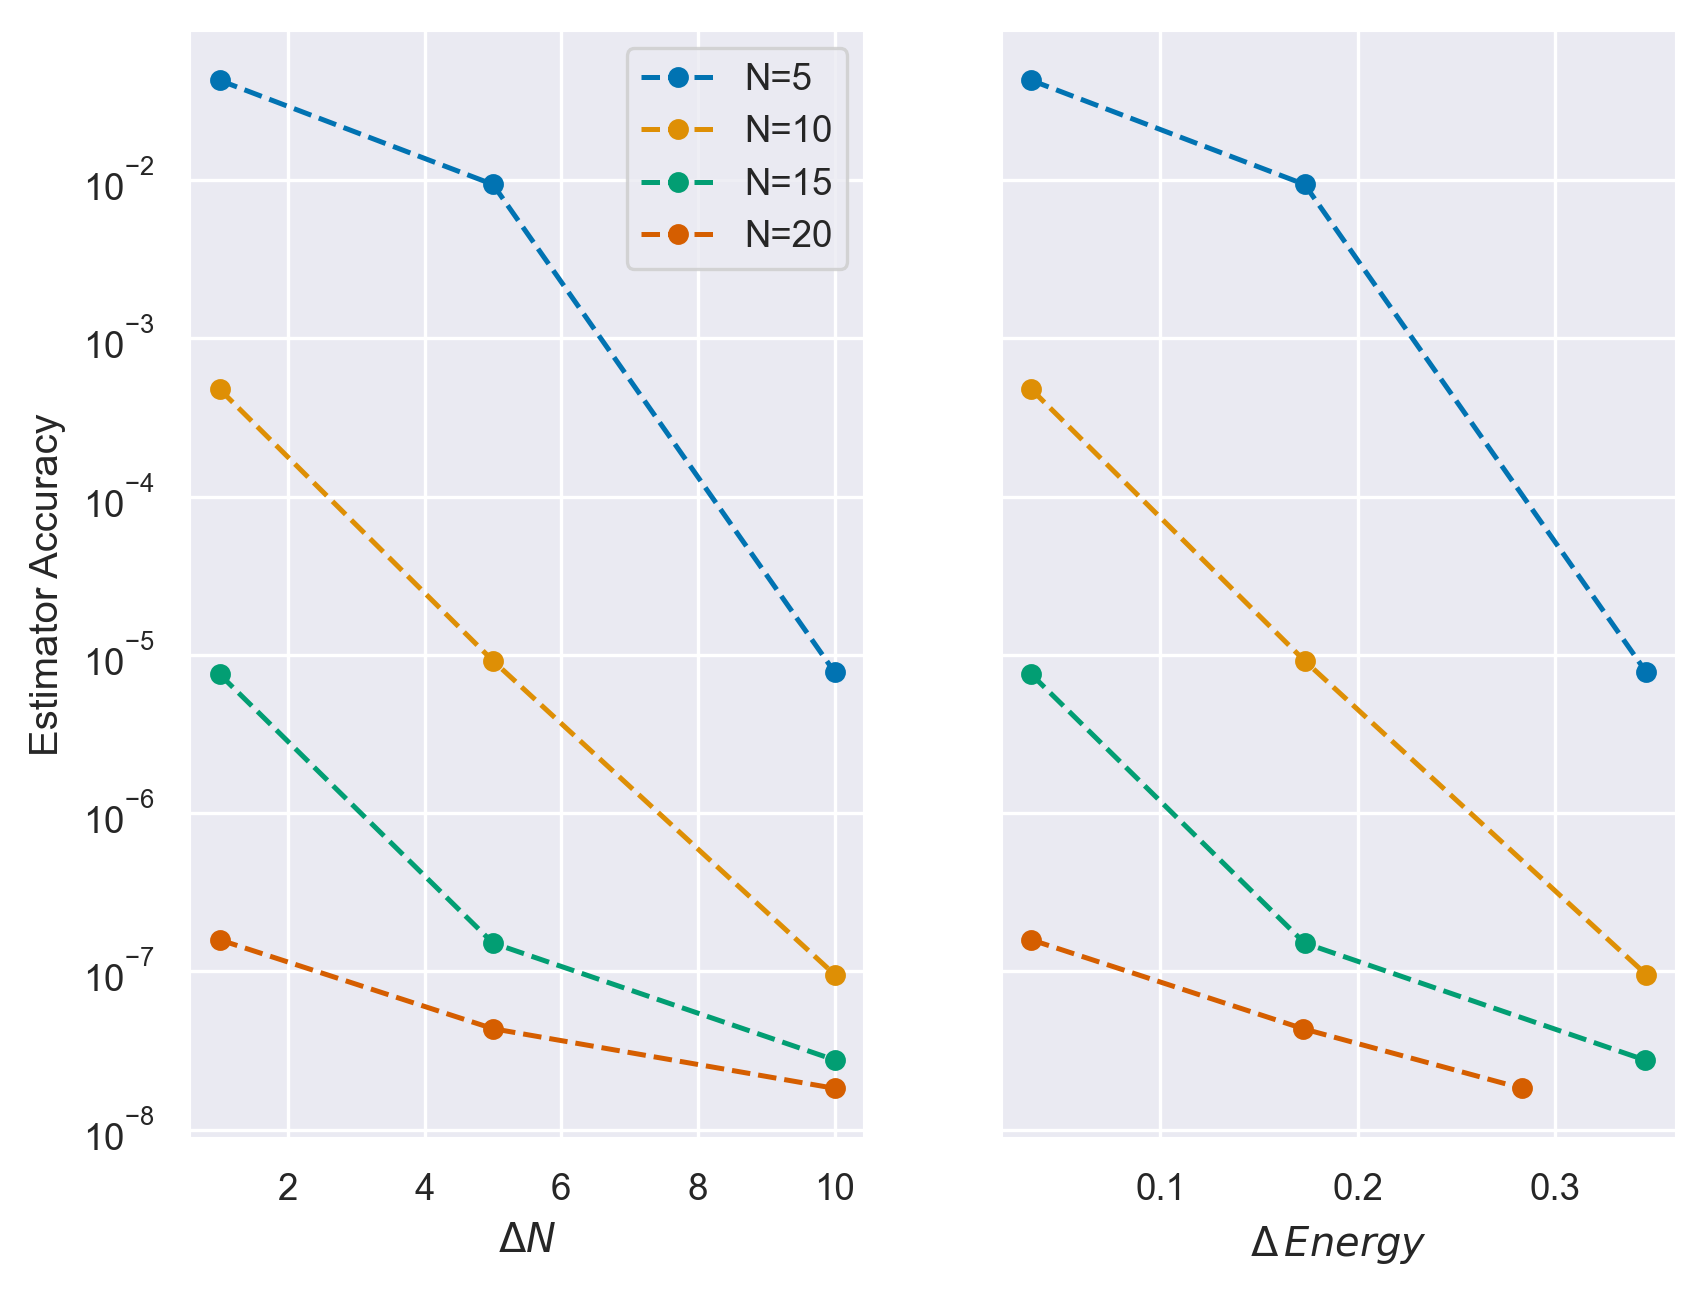
\includegraphics[width=1\columnwidth]{research_project/piston/figures/rb_certification/estimator_accuracy.png}
    \caption{A posteriori error estimator accuracy.
    We see how it can become more effective to carry more additional modes than rather just one.}
    \label{fig:estimator_accuracy}
\end{figure}
We conclude that it seems to be better to carry more than one mode.
Nevertheless, if it is going to become too costly to compute all these additional modes,
one extra mode could do the job fairly well too, provided that the base ROM is well resolved.

\end{document}